\subsection{GPU moments}
\label{sec:locate:gpu-moments}

From the previous approach, it was noticed that computing the moments on the different bubbles was a highly parallelizable task.
In fact, the same \texttt{moments} function was called for each bubble found by \texttt{FindContours}.

On top of that, the \texttt{moments} function used to compute moments up to order 3 (for a total of 24 moments), while only moments of order 0 and 1 were used.
As such, a tailored, GPU implementation was created to compute the centroids of the bubbles.
The resulting implementation was also extended to process contours of multiple cameras at the same time,  as well as considering more frames of the same camera in a batch.

\subsubsection{Algorithm}

\begin{enumerate}
	\itemsep 0em
	\item Through \texttt{OpenCV}'s \texttt{FindContours}, find all the bubbles for a given frame;
	\item Find the largest contour among them (this allows all GPU threads to work on the same data size, to avoid diversions);
	\item For each contour found, a GPU thread runs the following kernel:
	      \begin{enumerate}
		      \item Iterate over all pixels, accumulating $M_{00}$, $M_{01}$ and $M_{10}$;
		      \item Use the moments to compute the centroids;
		      \item Add the coordinates to the output list.
	      \end{enumerate}
\end{enumerate}

\subsubsection{Evaluation}

Since the algorithm the exact porting of the corresponding CPU algorithm, the output is the same (figure~\ref{fig:locate:moments}, 99\% of bubbles found).

For the speed evaluation, some tests were conducted to find the best, if any, batch size.
Figure~\ref{fig:locate:moments-cpu-vs-gpu} compares the speed of the CPU algorithm to the speed of the GPU algorithm, with respect to the total number of frames the GPU algorithm processes together.
In particular, this number corresponds to the product between the number of cameras and the batch size per camera.
It is visible that the GPU algorithm is faster, provided that at least 5 frames are processed concurrently, while reaching plateau performance when 10 frames are considered at each iteration.
For the final evaluation, we chose a batch size of 20 per camera, leading to 80 frames processed at the same time by the GPU.

While increasing this batch size adds a delay on the output, this delay only produces a one-time latency, not accumulating over time.
This is acceptable according to the project requirements, which allow for some processing latency, while requiring real-time regime speed.

The maximum speed achieved for this approach was 73 FPS, making this the fastest approach among all, but still not fully reaching the real-time target.

\begin{figure}
	\centerline{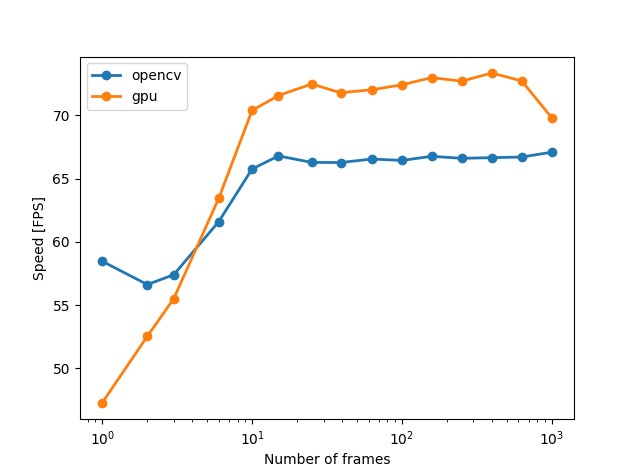
\includegraphics[width=.6\textwidth]{images/moments_opencv_vs_gpu.png}}
	\caption{\centering Comparing speed between CPU and GPU Image Moments algorithms with respect to number of frames processed.}
	\label{fig:locate:moments-cpu-vs-gpu}
\end{figure}
